\documentclass[11pt,a4paper]{article}

% ---------------------------------------------------------------------------
%  Guest Review Intelligence & Action Management System -- Final Module Report
% ---------------------------------------------------------------------------

% --- Typography: professional serif (Palatino-like) ---
\usepackage[T1]{fontenc}
\usepackage[utf8]{inputenc}
\usepackage{newpxtext}
\usepackage{newpxmath}
\usepackage{microtype}

% --- Layout ---
\usepackage[a4paper,margin=1in]{geometry}
\usepackage{setspace}
\setstretch{1.08}
\usepackage{enumitem}
\setlist{itemsep=2pt,topsep=3pt,parsep=0pt}
\usepackage{parskip}

% --- Graphics, tables, colour ---
\usepackage{graphicx}
\usepackage{booktabs}
\usepackage{array}
\usepackage{tabularx}
\usepackage{xcolor}
\usepackage{caption}
\captionsetup{font=small,labelfont=bf,skip=6pt}
\usepackage{amsmath}

% --- Section styling ---
\usepackage{titlesec}
\titleformat{\section}{\large\bfseries}{\thesection}{0.6em}{}
\titleformat{\subsection}{\normalsize\bfseries}{\thesubsection}{0.6em}{}
\titlespacing*{\section}{0pt}{14pt}{6pt}
\titlespacing*{\subsection}{0pt}{10pt}{4pt}

% --- Diagrams ---
\usepackage{tikz}
\usetikzlibrary{arrows.meta,positioning,fit,backgrounds,calc}

% --- Header/footer ---
\usepackage{fancyhdr}
\pagestyle{fancy}
\fancyhf{}
\renewcommand{\headrulewidth}{0.3pt}
\fancyhead[L]{\small Guest Review Intelligence \& Action Management}
\fancyhead[R]{\small The Kingsbury, Colombo}
\fancyfoot[C]{\small \thepage}

% --- Hyperlinks (blue links in the reference section) ---
\usepackage[colorlinks=true,linkcolor=black,citecolor=blue,urlcolor=blue]{hyperref}
\usepackage[round]{natbib}
\bibliographystyle{plainnat}

% --- Theme colours ---
\definecolor{navy}{HTML}{1F3A5F}
\definecolor{teal}{HTML}{2C7A7B}
\definecolor{lightgray}{HTML}{EEF2F6}
\definecolor{midgray}{HTML}{6B7280}

% --- Screenshot placeholder: uses real file if present, else a labelled box ---
\newcommand{\screenshot}[3]{%
  % #1 = filename (in figures/), #2 = caption, #3 = label
  \begin{figure}[t]
  \centering
  \IfFileExists{figures/#1}{%
    \includegraphics[width=0.92\linewidth]{figures/#1}%
  }{%
    \fcolorbox{midgray}{lightgray}{%
      \begin{minipage}[c][4.2cm][c]{0.9\linewidth}
        \centering
        {\large\bfseries\color{midgray} [ Screenshot placeholder ]}\\[4pt]
        {\color{midgray}\ttfamily figures/#1}\\[6pt]
        {\small\color{midgray} #2}
      \end{minipage}}%
  }
  \caption{#2}
  \label{#3}
  \end{figure}
}

% ===========================================================================
\begin{document}

% --------------------------- COVER PAGE ------------------------------------
\begin{titlepage}
\thispagestyle{empty}
\centering
\vspace*{1.2cm}
{\color{navy}\rule{\linewidth}{1.4pt}}\\[0.6cm]
{\Huge\bfseries Guest Review Intelligence\\[4pt] \& Action Management System}\\[0.5cm]
{\Large A Reputation-Protection Platform for The Kingsbury, Colombo}\\[0.3cm]
{\color{navy}\rule{\linewidth}{1.4pt}}\\[1.0cm]

{\large Final Module Report}\\[0.2cm]
{\itshape Turning thousands of scattered guest reviews into a prioritised,\\ department-owned action list, before problems define the brand.}\\[1.6cm]

\begin{tabular}{rl}
\textbf{Module} & \rule{6cm}{0.4pt} \\[10pt]
\textbf{Team / Authors} & \rule{6cm}{0.4pt} \\[10pt]
 & \rule{6cm}{0.4pt} \\[10pt]
\textbf{Institution} & \rule{6cm}{0.4pt} \\[10pt]
\textbf{Date} & June 2026 \\
\end{tabular}

\vfill
{\small\color{midgray} A working proof-of-concept built on live analysis of real Kingsbury reviews crawled
from Google, TripAdvisor and Booking.com, augmented with engineered incident fixtures.
Hotel financial figures are illustrative and explicitly flagged.}
\end{titlepage}

% --------------------------- ABSTRACT --------------------------------------
\begin{abstract}
\noindent
A five-star hotel's reputation is no longer written only by its front desk. Increasingly it is
mediated by algorithms, such as search rankings and conversational AI assistants, that read guest
reviews and distil them into a one-line verdict. When a recurring complaint is repeated by enough
guests it becomes a permanent caveat in how the property is described on every query. The Kingsbury,
Colombo, a five-star hotel rated 4.0/5 and ranked \#32 of 103 hotels in Colombo on TripAdvisor,
illustrates the problem. Thousands of reviews are spread across multiple platforms, far beyond what
any operations team can read, cross-reference and act on consistently.
This report presents a working proof-of-concept that runs the same mechanism that judges the hotel,
but \emph{for} the hotel. A multi-platform ingestion layer feeds a natural-language analysis pipeline
that scores every review for sentiment and a 0--100 reputation-risk value. A three-pass
large-language-model pipeline (Google Gemini~2.5~Flash) then distils negative and mixed reviews into a
small set of concrete, evidence-grounded, department-owned operational issues while preserving the
guest's exact specifics such as room number, amount and time. Across an analysed corpus of 2{,}939
reviews (weighted toward the reputation-relevant negative and mixed reviews), 2{,}294 problem reviews
collapsed into 117 active issues, roughly a 20:1 reduction, alongside 587 single-mention early-warning
signals, at a marginal detection cost of about US\$0.25 per full run. The report also addresses the
commercial dimensions of the system. These cover the authenticity of review data, the
hotel's true booking and review volumes, a defensible and bounded estimate of the room revenue exposed
to online reputation, and a concrete pricing model. We conclude that even on conservative assumptions
the platform protects a multiple of its cost, and we outline the path to production through incremental
detection and property-management-system integration.
\end{abstract}

\tableofcontents
\thispagestyle{fancy}
\newpage

% =========================================================================
\section{Introduction}

\subsection{Background}
Travellers no longer scroll through thousands of reviews before choosing a hotel. They ask a search
engine or an AI assistant a direct question, such as \textit{``Is The Kingsbury Colombo a good
hotel?''}, and receive a synthesised answer drawn from exactly those reviews. That answer typically
carries a caveat along the lines of \textit{``well-regarded, though some guests mention dated rooms,
noise from live music, and occasional service inconsistency.''} The caveat is not an opinion. It is a
problem that surfaced in reviews, was repeated by enough guests, and became baked into how the property
is described on every subsequent query. Online reputation has therefore become a direct commercial
asset. Cornell's analysis of lodging performance found that a one-percent improvement in a hotel's
online reputation score is associated with a 1.42\% increase in revenue per available room (RevPAR)
\citep{anderson2012social}, and more than 80\% of travellers read reviews before booking
\citep{tripadvisor2019reviews,reputationdefender2023stats}.

\subsection{Motivation}
The mechanism that now judges the hotel, an AI reading its reviews, is precisely the mechanism a hotel
should run \emph{for itself}, but sharper and earlier. A generic assistant only reports that an issue
has \emph{already} bubbled up, and by then it is a public caveat that no tool can delete. The
opportunity is to detect each operational fault at its \emph{first} mention rather than its
two-hundredth, route it to the responsible department, and fix the cause before it spreads. This is not
review deletion or damage repair. It is a standing investment in the reputation the hotel has not yet
lost.

\subsection{Problem statement}
A high-volume property generates more reviews, across more platforms and languages, than any operations
team can read, de-duplicate, risk-rank and assign consistently. The cost is not the reading time. It is
the \emph{pattern that gets missed}, the single complaint today that is silently the two-hundredth of a
recurring fault. The core problem this project addresses is the \textbf{cognitive-load and synthesis
gap}, namely converting a continuous, multi-platform stream of unstructured reviews into a short,
prioritised, evidence-backed and department-owned list of actionable issues.

\subsection{Objectives}
\begin{enumerate}[label=\textbf{O\arabic*.}]
  \item To \textbf{ingest and normalise} guest reviews from multiple platforms (Google, TripAdvisor,
        Booking.com) into a single canonical store through modular, official-shaped connectors.
  \item To \textbf{analyse} each review for sentiment, owning department, and a transparent 0--100
        reputation-risk score.
  \item To \textbf{detect operational issues} by distilling negative and mixed reviews into a small set
        of concrete, de-duplicated, evidence-grounded issues that preserve the guest's specifics.
  \item To \textbf{prioritise and assign} each issue to a department with risk-based ranking, recurrence
        tracking, and human-in-the-loop resolution.
  \item To \textbf{evaluate the commercial case}, covering data validity, demand context, a bounded
        revenue impact, and a concrete pricing model, against a real five-star property.
\end{enumerate}

\subsection{Scope}
The deliverable is a functioning proof-of-concept (POC) running locally, comprising a web application,
an API, and a relational database. It uses official-shaped connectors with sample and crawled data
rather than live production credentials, and is sized for a single property. Production concerns such as
live platform authorisation, incremental detection at full scale, and property-management integration
are designed for but deliberately out of POC scope, and are discussed in Sections~\ref{sec:discussion}
and~\ref{sec:conclusion}.

% =========================================================================
\section{Related Work}

\textbf{Review mining and aspect-based sentiment analysis (ABSA).} Extracting opinions about specific
aspects of a product or service from free text is a well-studied task, and the SemEval ABSA shared
tasks established standard formulations for aspect-term extraction and polarity classification
\citep{pontiki2016semeval}. Classical ABSA, however, produces \emph{aspect categories} such as
``rooms'' or ``staff'' rather than the concrete, owner-assignable \emph{incidents} an operations team
can act on, and it rarely preserves the specifics, such as a room number or a billed amount, that make
a complaint a closeable work order.

\textbf{Online reputation and revenue.} The link between online reputation and hotel performance is
empirically established. \citet{anderson2012social} quantified the RevPAR elasticity used throughout
this report, and subsequent industry studies confirm that the large majority of travellers consult
reviews before booking on \emph{any} channel \citep{tripadvisor2019reviews,reputationdefender2023stats}.

\textbf{Commercial reputation and social-listening tools.} Existing platforms aggregate reviews and
present sentiment dashboards and word clouds. Their gap, for an operator, is threefold. They report
generic themes such as ``people mention food'' rather than specific issues such as ``breakfast buffet
ran empty by 9\,am''. They attach no \emph{ownership} or tracking. And they react to themes only once
those themes are already prominent. This project's contribution is the combination of hotel-specific
issue detection, evidence and specifics down to the room number, department ownership and tracking, and
early-warning detection of single-mention signals, powered by a modern large language model
\citep{google2025gemini} over locally-computed sentence embeddings \citep{reimers2019sbert}.

% =========================================================================
\section{System Design and Methodology}
\label{sec:design}

\subsection{Architecture overview}
The system is a three-tier application (Figure~\ref{fig:arch}). A \textbf{Next.js / React} web client
presents three operator screens, namely Dashboard, Reviews and Issues. A \textbf{FastAPI} service
exposes a REST API and houses the ingestion connectors, the natural-language analysis, and the
issue-detection pipeline. State is persisted in \textbf{PostgreSQL}. Heavy natural-language models run
locally, covering sentiment, zero-shot department classification, and sentence embeddings. Only the
issue-detection reasoning calls an external large language model (Google Gemini~2.5~Flash), with a
deterministic offline \emph{stub} provider available for development and testing.

\begin{figure}[t]
\centering
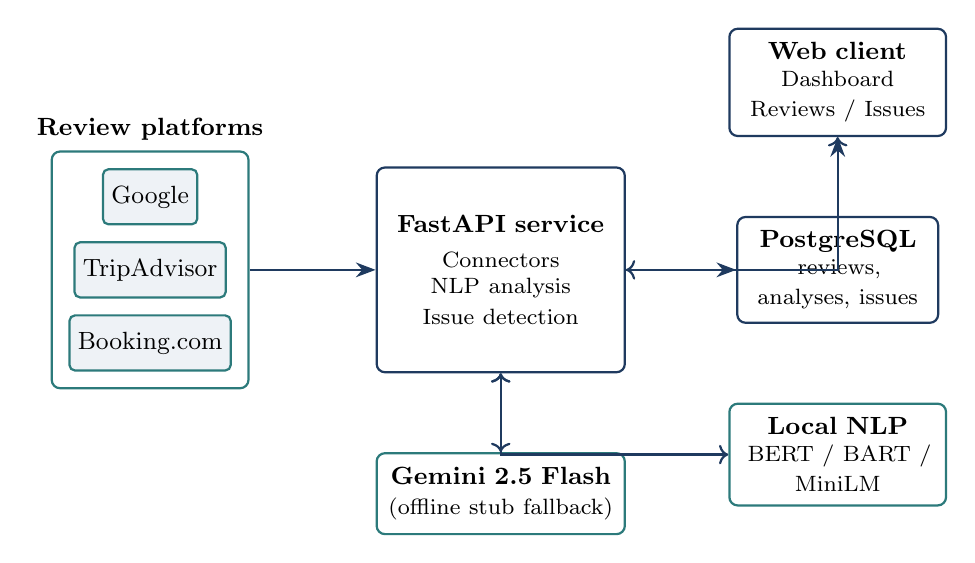
\begin{tikzpicture}[
  font=\small,
  box/.style={draw=navy,thick,rounded corners=3pt,align=center,minimum height=1.0cm,fill=white,inner sep=5pt},
  src/.style={draw=teal,thick,rounded corners=2pt,align=center,fill=lightgray,minimum height=0.7cm,inner sep=3pt},
  arr/.style={-{Stealth[length=2.5mm]},thick,navy}
]
% sources
\node[src] (g)  {Google};
\node[src,below=2mm of g]  (t)  {TripAdvisor};
\node[src,below=2mm of t]  (b)  {Booking.com};
\node[draw=teal,thick,rounded corners=3pt,fit=(g)(t)(b),inner sep=6pt,label=above:{\bfseries Review platforms}] (sources) {};
% api
\node[box,right=1.6cm of sources,minimum height=2.6cm,text width=2.8cm] (api)
  {\textbf{FastAPI service}\\[3pt]\footnotesize Connectors\\ NLP analysis\\ Issue detection};
% db
\node[box,right=1.4cm of api,text width=2.2cm] (db) {\textbf{PostgreSQL}\\\footnotesize reviews,\\ analyses, issues};
% web
\node[box,above=1.0cm of db,text width=2.4cm] (web) {\textbf{Web client}\\\footnotesize Dashboard\\ Reviews / Issues};
% llm
\node[box,below=1.0cm of api,text width=2.8cm,draw=teal] (llm) {\textbf{Gemini 2.5 Flash}\\\footnotesize (offline stub fallback)};
% local models
\node[box,below=1.0cm of db,text width=2.4cm,draw=teal] (loc) {\textbf{Local NLP}\\\footnotesize BERT / BART /\\ MiniLM};

\draw[arr] (sources) -- (api);
\draw[arr] (api) -- (db);
\draw[arr] (db) -- (web);
\draw[arr,<->] (web) |- (api);
\draw[arr,<->] (api) -- (llm);
\draw[arr,<->] (api) |- (loc);
\end{tikzpicture}
\caption{System architecture. Reviews flow from modular platform connectors into the FastAPI service,
which analyses them with local NLP models and an external LLM, persists results in PostgreSQL, and
serves the operator-facing web client.}
\label{fig:arch}
\end{figure}

\subsection{Ingestion and the canonical data model}
Each platform has a dedicated \textbf{connector} that accepts the platform's own (``official-shaped'')
payload and maps it to a canonical review. No scraping is required, and a source can be swapped without
touching the analysis engine. Raw payloads are preserved verbatim, with a content hash for idempotent
and duplicate-safe ingestion, and then normalised. The data model (Figure~\ref{fig:datamodel}) is a
linear enrichment pipeline. A raw review becomes a normalised review, which gains a one-to-one analysis
record, and may be linked as evidence to one or more detected issues.

\begin{figure}[t]
\centering
\resizebox{\linewidth}{!}{%
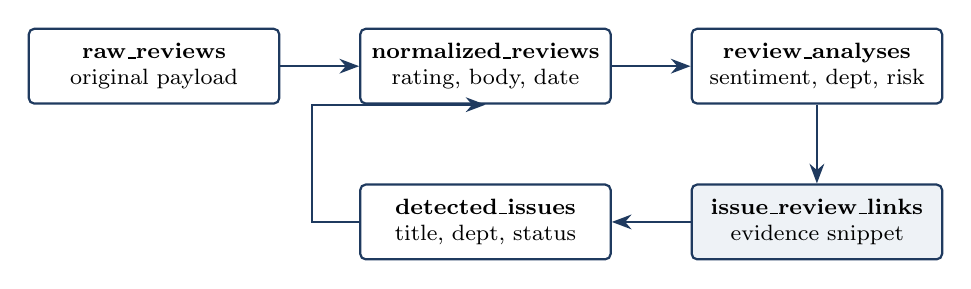
\begin{tikzpicture}[
  font=\small,
  ent/.style={draw=navy,thick,rounded corners=2pt,fill=white,align=center,minimum height=0.95cm,text width=2.9cm,inner sep=4pt,font=\footnotesize},
  arr/.style={-{Stealth[length=2.5mm]},thick,navy}
]
\node[ent] (raw) {\textbf{raw\_reviews}\\\footnotesize original payload};
\node[ent,right=1.0cm of raw] (norm) {\textbf{normalized\_reviews}\\\footnotesize rating, body, date};
\node[ent,right=1.0cm of norm] (an) {\textbf{review\_analyses}\\\footnotesize sentiment, dept, risk};
\node[ent,below=1.0cm of an,fill=lightgray] (link) {\textbf{issue\_review\_links}\\\footnotesize evidence snippet};
\node[ent,left=1.0cm of link] (iss) {\textbf{detected\_issues}\\\footnotesize title, dept, status};
\draw[arr] (raw) -- (norm);
\draw[arr] (norm) -- (an);
\draw[arr] (an) -- (link);
\draw[arr] (link) -- (iss);
\draw[arr] (iss.west) -- ++(-0.6,0) |- (norm.south);
\end{tikzpicture}}
\caption{Canonical data model. Reviews are progressively enriched, and issues are linked back to the
exact reviews and snippets that evidence them, giving every issue a traceable basis.}
\label{fig:datamodel}
\end{figure}

\subsection{Natural-language analysis}
Every normalised review is scored by three local models. The first is a multilingual BERT sentiment
classifier (positive, mixed or negative). The second is a zero-shot department classifier built on
BART-MNLI \citep{lewis2020bart} over six hotel departments (Front Office, Housekeeping, Food \&
Beverage, Engineering, Guest Relations, Management). The third is a MiniLM sentence-embedding model
\citep{reimers2019sbert} that produces a 384-dimensional vector used later for de-duplication and issue
clustering.

\paragraph{Reputation-risk score.} Each review receives a transparent, auditable 0--100 reputation-risk
score, labelled low, medium, high or critical, computed as a bounded sum of interpretable factors, so a
manager can see \emph{why} a review is urgent.
\begin{equation}
\text{risk} = \min\!\Big(100,\;
\underbrace{\tfrac{5-r}{4}\cdot 30}_{\text{rating}}
+ \underbrace{(-s)\cdot 25}_{\text{sentiment}}
+ \underbrace{w_d}_{\text{dept.}}
+ \underbrace{u}_{\text{urgency}}
+ \underbrace{v}_{\text{visibility}}
+ \underbrace{\rho}_{\text{recency}}
+ \underbrace{\delta}_{\text{duplicate}}\Big)
\label{eq:risk}
\end{equation}
Here $r$ is the star rating, $s\in[-1,1]$ the sentiment score, and $w_d$ a per-department weight
(Management highest). The term $u$ adds points for urgency words such as ``refund'', ``unsafe'' or
``manager'', $v$ for public visibility through helpful votes, a public URL or unanswered status, $\rho$
for recency, and $\delta$ for a detected duplicate. Every contributing factor is stored alongside the
score for audit.

\subsection{Issue detection through a three-pass LLM pipeline}
The core contribution is the issue-detection pipeline (Figure~\ref{fig:pipeline}), which runs only over
\textbf{negative and mixed} reviews, the reputation-relevant ones, in three passes.
\begin{description}[leftmargin=1.4em,style=nextline]
  \item[Pass A, Extract.] Reviews are sent to the LLM in small batches, and for each it returns a short
  problem summary, the owning department, and the concrete \emph{specifics} such as room or floor, item,
  amount and time.
  \item[Pass B, Consolidate.] All extracted problem labels are clustered into a \emph{dynamic} taxonomy
  of canonical issue types rather than a hard-coded list. Genuinely distinct severe incidents such as a
  pest sighting, theft or a safety hazard are deliberately kept separate rather than folded into a
  generic category.
  \item[Pass C, Assemble.] Each canonical type becomes one issue with an evidence-grounded description.
  A type supported by $\geq 2$ reviews becomes an \textbf{active} issue, while a single-mention type
  becomes an \textbf{emerging} early-warning signal. A stable \texttt{cluster\_key} lets the pipeline be
  re-run idempotently while preserving manual state such as assignee and resolved status.
\end{description}
The defining property is \textbf{specificity preservation}. The output is not ``billing problems'' but
``room~1413, US\$60 unexplained charge'', a closeable work order rather than a theme.

\begin{figure}[t]
\centering
\resizebox{\linewidth}{!}{%
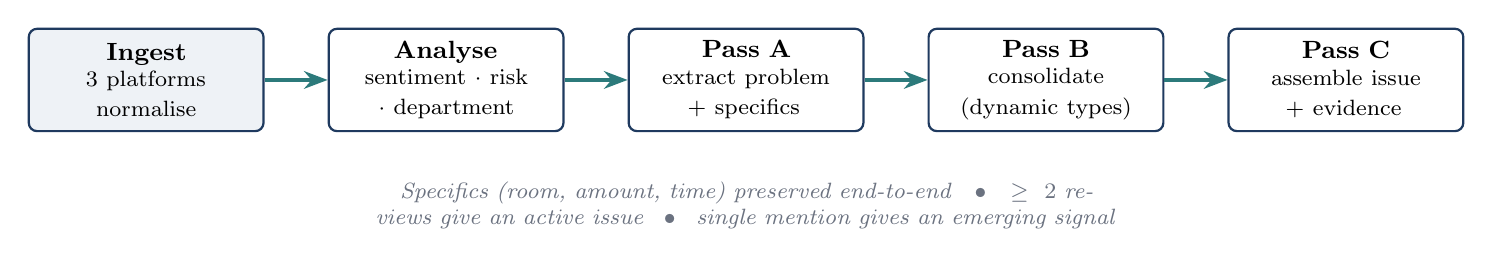
\begin{tikzpicture}[
  font=\small,
  stage/.style={draw=navy,thick,rounded corners=3pt,fill=white,align=center,minimum height=1.3cm,text width=2.7cm,inner sep=4pt},
  arr/.style={-{Stealth[length=3mm]},very thick,teal}
]
\node[stage,fill=lightgray] (ing) {\textbf{Ingest}\\\footnotesize 3 platforms\\ normalise};
\node[stage,right=0.8cm of ing] (an) {\textbf{Analyse}\\\footnotesize sentiment $\cdot$ risk\\ $\cdot$ department};
\node[stage,right=0.8cm of an] (a) {\textbf{Pass A}\\\footnotesize extract problem\\ + specifics};
\node[stage,right=0.8cm of a] (b) {\textbf{Pass B}\\\footnotesize consolidate\\ (dynamic types)};
\node[stage,right=0.8cm of b] (c) {\textbf{Pass C}\\\footnotesize assemble issue\\ + evidence};
\foreach \x/\y in {ing/an,an/a,a/b,b/c} \draw[arr] (\x) -- (\y);
\node[below=0.5cm of a,text width=10.5cm,align=center,font=\footnotesize\itshape,color=midgray]
  {Specifics (room, amount, time) preserved end-to-end $\;\bullet\;$
   $\geq 2$ reviews give an active issue $\;\bullet\;$ single mention gives an emerging signal};
\end{tikzpicture}}
\caption{The end-to-end pipeline. Reviews are ingested and analysed, then a three-pass LLM stage
extracts, consolidates and assembles concrete, evidence-grounded issues.}
\label{fig:pipeline}
\end{figure}

\subsection{Data and evaluation methodology}
\label{sec:data}
The analysed corpus comprises \textbf{2{,}939 reviews}. These combine \emph{real reviews crawled from
Google and TripAdvisor} for The Kingsbury with a set of \emph{engineered incident fixtures}. The corpus
was deliberately weighted toward \textbf{negative and mixed} reviews because those are the only
reputation-actionable inputs. The detection pipeline reads negative and mixed reviews exclusively, and
positive reviews yield no issues to act on. The engineered fixtures were generated from a library of
specific incident scenarios, each carrying concrete facts such as room, floor, item, amount and time,
precisely in order to \textbf{stress-test specificity preservation}. Real crawled reviews frequently
omit such details, so synthetic incidents let us verify that the pipeline carries a guest's exact facts
all the way through to the final issue. This is the principal validity caveat of the quantitative
findings and is discussed further in Section~\ref{sec:discussion}. The macro reputation picture, namely
the rating, ranking and dominant complaint themes, is corroborated by the real crawled reviews and by
independent public data.

% =========================================================================
\section{Results and Findings}

\subsection{Scale and compression}
Table~\ref{tab:scale} summarises the headline result. The 2{,}294 negative and mixed reviews collapsed
into 117 active issues, a roughly \textbf{20:1 compression}, so that managers act on 117 things rather
than reading thousands of complaints. A further 587 single-mention \emph{emerging} signals were caught
as early warnings, and 77\% of complaint reviews were traced to a concrete, fixable issue via 3{,}793
evidence links. The dashboard and issues screens (Figures~\ref{fig:dashboard} and~\ref{fig:issues})
surface these for the operations team.

\begin{table}[h]
\centering
\caption{Corpus and detection outcomes.}
\label{tab:scale}
\begin{tabularx}{\linewidth}{Xr}
\toprule
\textbf{Metric} & \textbf{Value} \\
\midrule
Reviews analysed (negative/mixed-weighted corpus) & 2{,}939 \\
Negative \& mixed (reputation-relevant) reviews & 2{,}294 \\
Active issues detected & 117 \\
Compression ratio (problem reviews to active issues) & $\approx$ 20:1 \\
Emerging (single-mention) early-warning signals & 587 \\
Complaint reviews traced to a concrete issue & 77\% (3{,}793 links) \\
Issues at critical risk ($\geq 80$) & 54 \\
Marginal LLM cost per full detection run & $\approx$ US\$0.25 \\
\bottomrule
\end{tabularx}
\end{table}

\screenshot{dashboard.png}{Dashboard showing the KPI cards (sentiment mix, risk distribution, and
active, high-risk and recurred issue counts) with sentiment and risk donuts and per-department issue
bars.}{fig:dashboard}

\subsection{The issues that matter}
Table~\ref{tab:issues} lists the highest-impact detected issues. The single most-complained-about
problem, loud music and event noise with 201 mentions at risk~89, is \emph{exactly} the caveat a
conversational AI repeats about the hotel, which confirms that the system measures the same signal the
market already reads. Critically, issues arrive with receipt-level specificity. Billing complaints are
not a generic category but, for example, ``room~1413, US\$60 unexplained charge'', a work order the
front office can close immediately.

\begin{table}[h]
\centering
\caption{Top detected issues (verbatim from the system).}
\label{tab:issues}
\begin{tabularx}{\linewidth}{Xrcl}
\toprule
\textbf{Issue} & \textbf{Mentions} & \textbf{Risk} & \textbf{Owner} \\
\midrule
Loud music / event noise disturbance & 201 & 89 & Management \\
Air conditioning fails to cool rooms  & 174 & 74 & Engineering \\
Long wait at check-in / check-out     & 169 & 85 & Front Office \\
Breakfast buffet not replenished      & 136 & 72 & Food \& Beverage \\
Incorrect / unexplained charges on bill & 122 & 82 & Front Office \\
Slow / unstable WiFi                  & 114 & 85 & Engineering \\
Poor food quality                     & 113 & 85 & Food \& Beverage \\
\bottomrule
\end{tabularx}
\end{table}

Active issues distribute across owners as Food \& Beverage~37, Front Office~25, Engineering~25,
Housekeeping~15, Management~9 and Guest Relations~6, for 117 in total, giving each department head a
self-contained, ranked queue.

\screenshot{issues.png}{Issues page showing the active-issue queue with title, owning department,
status, priority, reputation-risk score and assignee. An ``Emerging candidates'' tab holds the 587
single-mention signals.}{fig:issues}

% =========================================================================
\section{Business and Market Analysis}
\label{sec:business}

This section examines the commercial case for the system, covering review authenticity, the hotel's
true demand and review volumes, a defensible revenue impact, and pricing.

\subsection{Review authenticity and data validity}
\label{sec:authenticity}
A fair objection is that anyone can post a review claiming a specific room had a fault, and that the
hotel's own property-management system (PMS) is the authoritative record of who stayed where.
We make three points. First, two of the three sources are \textbf{verified-stay channels}. On
Booking.com and, predominantly, TripAdvisor, reviews originate from guests with a booking, which
constrains fabrication, whereas Google is the open channel and is treated as lower-confidence. Second,
and more fundamentally, \textbf{authenticity is not the problem this system solves}. Its purpose is to
reduce the cognitive load of monitoring a high-volume, multi-platform review stream and to surface
recurring, reputation-damaging patterns early. A pattern of 201 independent guests reporting noise is
meaningful \emph{regardless} of any single review's provenance, because the signal is in the
aggregation rather than the individual post. Third, the system never acts autonomously. Every issue
carries its evidence and a confidence score, and a human resolves or dismisses it. \emph{The system
proposes, and staff decide.} Integrating the PMS, so as to corroborate a complaint against the actual
folio for room~1413 on a given night and turn a flagged issue into a verified one, is a high-value
enhancement, but it requires hotel-internal access and is therefore planned as production work rather
than POC scope (Section~\ref{sec:conclusion}).

\subsection{Demand and review context, would the hotel care?}
\label{sec:demand}
To judge materiality we size the hotel's demand using its real room count of 229 and clearly-flagged
illustrative operating assumptions (Table~\ref{tab:demand}). At a representative 72\% occupancy and a
US\$130 average daily rate, the property turns roughly 60{,}000 occupied room-nights and about
US\$7.8\,M of room revenue per year, and at an estimated average stay of about 2.5 nights it sees on the
order of 65 arrivals per day. Against its roughly 20{,}000 cumulative public reviews, current review
velocity is on the order of 10 to 20 new reviews per day across platforms. These are not large numbers
to \emph{read}, which is the heart of a natural objection, that a staff member could simply read them. But
reading is not the task. The task is \emph{synthesis}, namely connecting one complaint today to the two
hundred spread across twelve months, three platforms and several languages, scoring each consistently,
and spotting the one emerging issue among hundreds. That is what no human team sustains, and it is what
the 20:1 compression and 587 early-warning signals deliver.

\begin{table}[h]
\centering
\caption{Demand context for The Kingsbury. The room count of 229 is real, and operating ratios are
illustrative benchmarks, flagged as such.}
\label{tab:demand}
\begin{tabularx}{\linewidth}{Xr}
\toprule
\textbf{Quantity} & \textbf{Estimate} \\
\midrule
Rooms (actual) & 229 \\
Assumed occupancy (illustrative) & 72\% \\
Assumed average daily rate (illustrative) & US\$130 \\
Occupied room-nights / year & $\approx$ 60{,}200 \\
Room revenue / year (illustrative) & $\approx$ US\$7.8\,M \\
Arrivals / day (at $\sim$2.5-night stay) & $\approx$ 65 \\
Cumulative public reviews (all platforms) & $\approx$ 20{,}000 \\
Estimated new reviews / day & $\approx$ 10--20 \\
\bottomrule
\end{tabularx}
\end{table}

\subsection{Estimating the revenue impact}
\label{sec:revenue}
A naive estimate applies the Cornell elasticity, where +1\% reputation gives +1.42\% RevPAR
\citep{anderson2012social}, to the \emph{entire} US\$7.8\,M room revenue, giving about US\$111k per 1\%
of reputation protected. That figure overstates the effect, because not all revenue responds to online
reputation. A portion of bookings comes through offline channels such as corporate accounts, travel
agents and walk-in. We therefore estimate the impact against only the revenue base that online
reputation plausibly influences, and we present a \textbf{range} rather than a single number
(Table~\ref{tab:revenue}).

The bounds are reasoned as follows. The \emph{floor} attributes impact only to OTA-booked room-nights.
In Asia, OTAs account for roughly 70\% of \emph{online} hotel bookings \citep{asia2024ota}, which for a
five-star city hotel with substantial direct and corporate business we take as about 25\% of
\emph{total} room-nights. The \emph{ceiling} recognises that review influence is not confined to OTA
bookings, because more than 80\% of travellers read reviews before booking on \emph{any} channel,
including the hotel's own website \citep{tripadvisor2019reviews,reputationdefender2023stats}, so
reputation shapes demand far beyond the OTA slice. The takeaway is not a single dramatic number but a
robust one. \textbf{Each 1\% of reputation protected is worth roughly US\$28k to US\$89k per year},
with a midpoint near US\$60k, and the elasticity cuts both ways, so this is also the revenue \emph{at
risk} from a 1\% erosion.

\begin{table}[h]
\centering
\caption{Bounded annual value of protecting 1\% of online reputation. The Cornell elasticity is applied
to the review-influenced revenue base, and all hotel financials are illustrative.}
\label{tab:revenue}
\begin{tabularx}{\linewidth}{Xccc}
\toprule
\textbf{Scenario} & \textbf{Influenced base} & \textbf{Revenue base} & \textbf{Value / 1\%} \\
\midrule
Floor (OTA room-nights only)        & $\approx$25\% & $\approx$US\$2.0\,M & $\approx$US\$28k \\
Mid (all online bookings)           & $\approx$55\% & $\approx$US\$4.3\,M & $\approx$US\$61k \\
Ceiling (all review-influenced demand) & $\approx$80\% & $\approx$US\$6.3\,M & $\approx$US\$89k \\
\bottomrule
\end{tabularx}
\end{table}

\subsection{Cost analysis and pricing}
\label{sec:pricing}
The platform is inexpensive to run. The dominant marginal cost is the LLM detection run at about
US\$0.25 over roughly 1{,}000 reviews, and even run daily that is under US\$100 per year. Local NLP
models run on commodity hardware at no per-use cost, and infrastructure for a single property is modest.
Table~\ref{tab:cost} sets out the proposed commercial model.

\paragraph{Recommended model, a one-time licence plus support.} The hotel pays a one-time product and
implementation licence, a small monthly support fee, and the very low runtime cost directly. This suits
a single flagship property that prefers a capital purchase over an open-ended subscription, and it keeps
the vendor's incentives aligned with reliability rather than usage. \emph{An alternative we considered
is an annual SaaS fee}, a flat per-property annual charge with runtime folded in, which is simpler to
budget and better for a multi-property rollout, and it is listed here as the secondary option.

\begin{table}[h]
\centering
\caption{Proposed pricing under the recommended model, with indicative figures.}
\label{tab:cost}
\begin{tabularx}{\linewidth}{Xr}
\toprule
\textbf{Component} & \textbf{Indicative} \\
\midrule
One-time product licence + implementation & $\approx$US\$9{,}500 \\
Monthly support \& maintenance & $\approx$US\$200 / month \\
LLM runtime (paid by hotel, daily runs) & $<$US\$100 / year \\
\midrule
Year-1 total (illustrative) & $\approx$US\$12{,}000 \\
Ongoing annual (support + runtime) & $\approx$US\$2{,}500 \\
\bottomrule
\end{tabularx}
\end{table}

\paragraph{Return on investment.} Even on the conservative floor of Table~\ref{tab:revenue}, protecting
just half a percent of reputation is worth about US\$14k per year, which is above the year-one cost, and
on the midpoint the platform pays for itself many times over. Because the value scales with revenue
protected while the cost is near-fixed, the return is order-of-magnitude rather than marginal.

% =========================================================================
\section{Discussion, Limitations, Risks and Mitigations}
\label{sec:discussion}

\paragraph{Synthetic-data validity.} The clearest limitation is that the quantitative corpus is
augmented with engineered incident fixtures (Section~\ref{sec:data}), so the absolute issue counts
should be read as a demonstration of the pipeline's behaviour at scale rather than as a precise census
of The Kingsbury's faults. The augmentation was a deliberate methodological choice to test specificity
preservation, and the dominant themes are corroborated by real crawled reviews. A full production run
over the hotel's complete real review history is the natural next step.

\paragraph{Other risks and their mitigations} are summarised in Table~\ref{tab:risk}.

\begin{table}[h]
\centering
\caption{Key risks and mitigations.}
\label{tab:risk}
\renewcommand{\arraystretch}{1.25}
\begin{tabularx}{\linewidth}{>{\bfseries}p{3.4cm}X}
\toprule
\textnormal{\textbf{Risk}} & \textbf{Mitigation} \\
\midrule
Data-source dependency & Official-shaped, modular connectors with no scraping. A source can be swapped
without touching the detection engine. \\
LLM cost at scale & The pipeline already stores a cluster centroid per issue, which enables
\emph{incremental} detection. New reviews are matched to existing clusters cheaply and the LLM is called
only for genuinely novel problems, so cost tracks new volume rather than total history. \\
Detection accuracy and false positives & Every issue is evidence-linked and confidence-scored with
human-in-the-loop resolve or dismiss. The system proposes, and staff decide. \\
Adoption (``another dashboard'') & The output is a prioritised, department-owned action list that fits
existing operations rather than a raw feed, with near-zero cost to trial. \\
\bottomrule
\end{tabularx}
\end{table}

% =========================================================================
\section{Conclusion and Future Work}
\label{sec:conclusion}

This report presented a working proof-of-concept that turns a high-volume, multi-platform stream of
guest reviews into a short, prioritised, evidence-grounded and department-owned list of operational
issues. On an analysed corpus of 2{,}939 reviews the system compressed 2{,}294 problem reviews into 117
active issues, a roughly 20:1 reduction, plus 587 early-warning signals, at a marginal cost of about
US\$0.25 per run, while preserving the guest's exact specifics down to room numbers and billed amounts.
We grounded the commercial case in bounded, sourced figures. These covered
verified-stay data with human-in-the-loop validation, a realistic demand and review-velocity picture, a
revenue impact of roughly US\$28k to US\$89k per 1\% of reputation protected against a year-one cost
near US\$12k, and a concrete one-time-licence-plus-support pricing model.

The principal next steps are a full detection run over the hotel's complete real review history, the
incremental-detection path that bounds LLM cost at production scale, PMS integration to corroborate
complaints against actual folios and convert flagged issues into verified ones, and multi-property
support to amortise the platform across a hotel group. The core thesis stands. A hotel cannot delete
what an algorithm has already learned about its past, but for cents per analysis it can ensure
tomorrow's problems never become the next permanent caveat.

% =========================================================================
\bibliography{references}

\end{document}
